\chapter{背景}
\label{background}

本章では本研究の背景について述べる.
まず機械学習における活性化関数のの役割について明確にする。
活性化関数について概説し、現在の機械学習における活性化関数の抱える問題点を明らかにする。
次に、活性化関数の他に、ニューラルネットワークにおける精度を向上させるいくつかの構成要素について述べる。
本研究の問題点の解決に必要な、ノンパラメトリックモデルとその具体例であるカーネル法を導入する。
また、統計学において活性化関数に相当する概念がどのように応用されてきたか述べる。
最後に、実社会において機械学習を行う上での問題点や課題を述べ、本研究が取り組むべき課題を明確にする。



\section{活性化関数}

\begin{figure}[hbtp]
    \begin{center}
        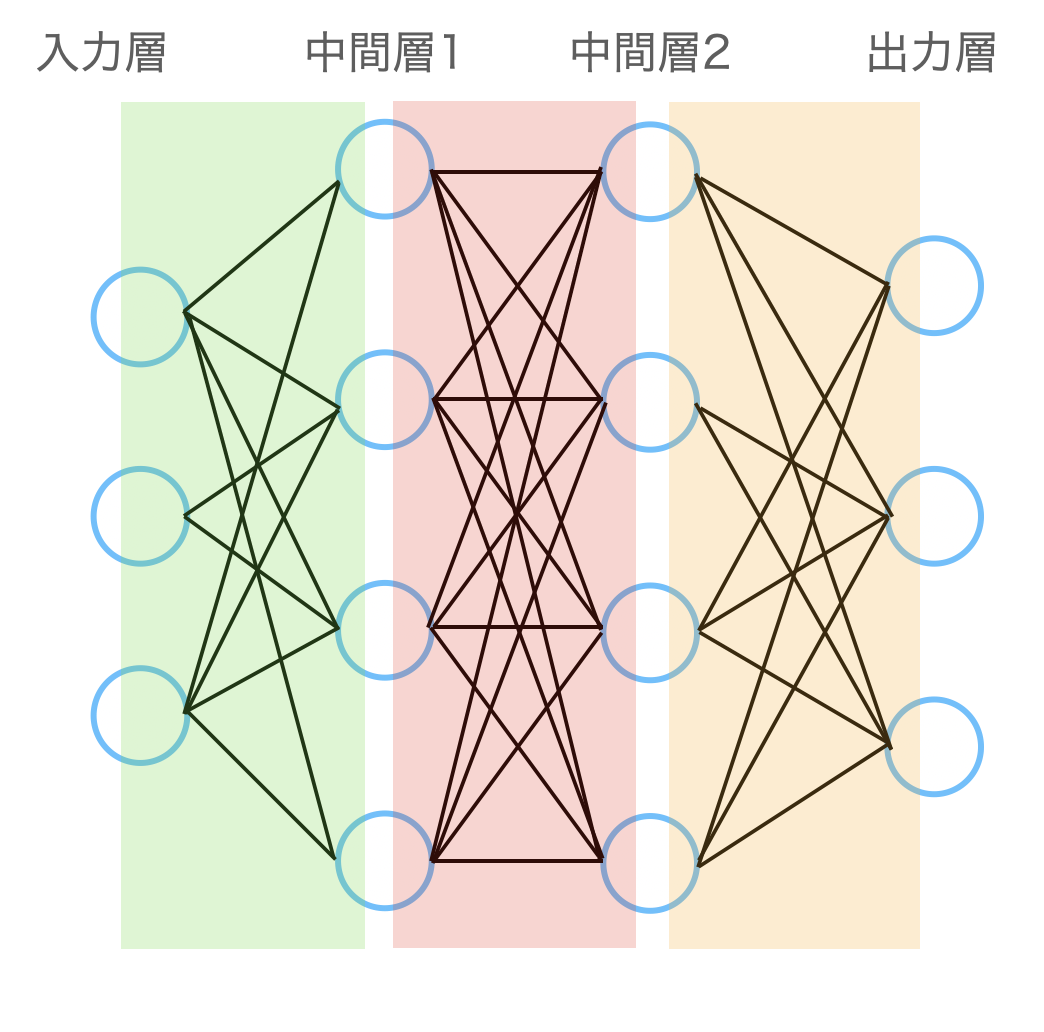
\includegraphics[width=10cm]{asset/neural_network1.png}
            \caption{活性化関数の形}
            \label{neural_network1}
    \end{center}
\end{figure}

また、概要を述べるにあたってニューラルネットワークの用語を定義する。活性化関数は
図の黄色で囲った活性化関数を出力層の活性化関数、赤色部分を中間層の活性化関数、緑色部分を入力そうの活性化関数と呼ぶことにする。

ディープラーニングの活性化関数に関する最近の研究はまだ多く、様々な実験が 行われている。~\cite{study_af}
活性化関数の歴史はシグモイドという脳のニューロンの数学的モデルに基づいた関数を応用したものにはじまる。
ニューラルネットワークの層に活性化関数を適用する過程を以下に示す。
$ w_i$ を重み、$ x_i $ は入力の値、$ b $はバイアス、$z$ は出力、$ g $ を活性化関数とした時
$ z=g(y)=g(\sum w_i x_i+b) $ 
このように用いられる。
その後TanhやReLUなどといったより計算に適した活性化関数が発見されてきた。
特にReLUに関しては現在のディープラーニングなどの深層ニューラルネットワークにおいても未だ応用されており、実用的にもその有用性が示されていることがわかる。

長年にわたり、性能を向上させ、ReLUの欠点に対処する多くの活性化関数が提案されてきたが、その中にはLeaky ReLU ~\cite{leaky_relu}、ELU~\cite{elu}、SELU~\cite{selu}などが含まれる。
Swish~\cite{swish}は、$ f(x)=x {\bf sigmoid(\beta x)} $ と定義できるが、よりロバストな活性化関数であることが証明され、ReLUと比較して結果が大幅に改善された。
活性化関数はそれまで単調増加な関数が使われることが多かったが、Swishで単調増加である必要なく、汎用的に精度が向上することがわかった。
またそのような活性化関数の例としてMishと言うものもあげらている。~\cite{Mish}

~\cite{trend_af}~\cite{evo_af}~\cite{study_af}~\cite{parametric_af}~\cite{isotron}~\cite{efficient_sim}~\cite{lsim}~\cite{sim}~\cite{ichimura}~\cite{Evolving}~\cite{swish}~\cite{resnte}~\cite{sim}

\begin{table}[htbp]
    \begin{center}
        \caption{活性化関数の種類}
        \label{class_af}
        \begin{tabular}{cp{5cm}cc}
        活性化関数の数式              & 数式 \\
        \hline
        Sigmoid            & sigmoid(x) \\
        Tanh               & tanh(x) \\
        ReLU        &  \[l=
            \begin{cases} 
            0 &\text{when x < 0 }\\
            x &\text{when x \lq 0 else} \\
            \end{cases}
            \] & & \\
        Swish           & $ x{\bf sigmoid}(\beta x) $ \\
        Mish           & $ x{\bf tanh}(softplus(x)) $ \\

        \end{tabular}
    \end{center}
\end{table}



\section{勾配の消失}
勾配消失問題とは、ニューラルネットワークの設計において、勾配が消失することで学習が進まなくなる技術的な問題のことである。
Sigmoidなどの場合、勾配が0に近い領域が存在するため、勾配消失に陥ると重みがほぼ修正されなくなる。
多層ニューラルネットワークでは一カ所でも勾配が0に近い層が存在すると、それより下層の勾配も全て0に近くなることが知られている。
このため、層数が増えるほど学習が難しくなっていた。現在一般的に使われているReLUは勾配消失に陥りづらいと言うところが精度向上につながっている。



\section{汎用的な活性化関数}

しかしながら、\ref{class_af}であげたような活性化関数は、どれも実験的に精度が向上すると言う理由で選択したものであり、あらゆるパターンにおいて最適かどうかと言う議論がされていない。
また、Alberto Marchisio~\cite{automatic_af}は、このような問題を解決するため、既存の活性化関数の中から最適な活性化関数を見出しています。
しかし、その選択は、すでに知られているものから関数全体を選択している。Garrett Bingham(2020)は、内部から探索することはできなかったようです。
多くのハイパーパラメータを持つ活性化関数を選択し、訓練で推定することで精度が向上します。 しかし、これも関数全体の探索には程遠い。
より良い活性化関数を選択して精度を向上させ、パラメータ数を減らすことは、より良いモデルを学習・発見するための重要な課題である。




\section{統計学における位置付け}

\begin{figure}[hbtp]
        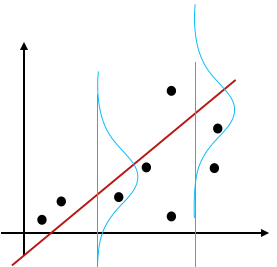
\includegraphics[width=6cm]{asset/glm1.png}~~~~~ ~~~~~ 
        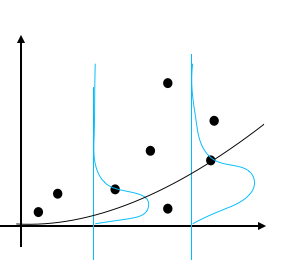
\includegraphics[width=6cm]{asset/glm2.png}
            \caption{活性化関数の形}
            \label{neural_network1}
\end{figure}

\subsubsection{一般線形化モデルとは}
 一方、統計学の世界に目を向けると、活性化関数と同様の概念がリンク関数(Link Function)として一般化線形モデル(GLM)においても流用されている。
説明変数を$ X $, パラメータを$ w $で表現し、従属変数を$ Y $とすると、$ \epsilon \sim \mathcal{G}(0, \sigma^2) $

$ Y = X \cdot w + \epsilon $
線形モデルの数式は$ E[Y] = X\cdot w $で表現することができる。
しかしながら、このままでは従属変数が正規分布に従わない場合に徐々に誤差が生まれてしまう。

GLMの数式はリンク関数$ G $を用いて以下のように示す。

\begin{eqnarray}
E[Y|X]=G^{-1} (X\dot w)
\end{eqnarray}

\subsubsection{シングルインデックスモデルとは}
シングルインデックスモデル(SIM)とは

GLM(Generalized Linear Model)やSIM(single index model)などの線形回帰の一般化が提案されている。

これら2つのモデルは、$ E[Y|X]=X\cdot w $の線形回帰モデルに、$ E[Y|X]=X\cdot w $のリンク機能を持たせたものです。 
統計学の世界では汎用的なリンク関数の提案としてisotonic regressionを応用した手法が研究されている。


 一方、SIMではリンク関数gの推定にノンパラメトリックな手法を用いており ディープラーニングには適用されていないようです。
 また、SIMの経験的に推定可能な反復学習 LPAVアルゴリズムと呼ばれるL-isotron法がSham Kakade~\cite{efficient_sim}で紹介されている。 
 しかし、LPAVでは線形相補的な位置推定法を用いてデータを並べ替えるため、ディープラーニングのような重い計算には不向きである。 

isotonic regressionはGLMと同様に推定する関数に単調増加性を仮定している。統計学の世界ではリンク関数自体が逆関数の考え方から導出されているため、
このように単調増加性を仮定しているが、これは必要のない仮定である。

\section{ノンパラメトリックモデルとカーネル法}

カーネル法とははパターン認識において使われる手法の一つで、 判別などのアルゴリズムに組み合わせて利用するものである。

 また、活性化関数に対応するリンク関数が未知の場合には、カーネル推定などのリンク関数をノンパラメトリックに推定する方法が市村(1993)によって提案されている。
 しかし、リンク関数をデータセット全体で推定するため、ディープラーニング的には データ数が多い場合でも有効ではない。
 Klein and Spadyの二項選択モデル~\cite{klein}も同様の手法である.

 カーネル関数を用いたノンパラメトリックな方法で提案されているが、この方法での深層学習については研究されていない。




\section{学習におけるいくつかの知識}
機械学習において精度を向上させる方法は大きく分けると
\subsection{ラーニングレート}
学習率はニューラルネットにおけるハイパーパラメータの一つ。入念に調整する必要がある。
\subsection{初期値}
ニューラルネットワークの学習効率は、重みの初期値によって大きく変わることが知られている。
初期値は0や1で初期化する方法以外にさまざまな方法がある。

\subsubsection{Uniform}
Uniform:-1.0~1.0の一様乱数で初期化します
\subsubsection{orthogonal}
\subsubsection{sparse}
sparseは~\cite{sim}で紹介されている。
2次元入力テンソルを疎な行列として充填し,ここで非ゼロ要素は,正規分布で埋める。
\subsubsection{kaiming uniform}
ガウス乱数にKaiming He提案の係数をかけて初期化する。

\subsection{レギュラライザー}
ニューラルネットワークは学習を行う際に、初期値やデータによっては重みに偏りが生まれ、勾配消失につながる可能性が高くなる。それらを解消するために、損失関数に数学的な項を加えることで学習の際の偏りを解消する手法が、実用的にも用いられている。
\subsubsection{L2ノルム}
ippanntek
\subsubsection{L1ノルム}

\subsection{optimizer}
この辺について



\section{実社会における学習の問題点}
ディープラーニングをGUIで簡易的に扱えるツールとして株式会社ソニーのNeural Network Consoleがある。
しかしながらそれでも共通として存在する問題点はデータセットの整形はこちら側でやる必要があるということである。
データ整形のプログラムは非技術者には難易度が高く
機械学習を導入するにあたって、データセットに応じたさまざまなメタ的要素の取捨選択が必要となり、
